In diesem Kapitel wird die zugrundeliegende Systemarchitektur vorgestellt, die sich im Wesentlichen in eine lokale Detektionsdomäne und eine globale P2P-Kommunikationsdomäne gliedert.

\section{Systemüberblick und verteilte Kommunikation}
\label{sec:systemueberblick_und_verteilte_Kommunikation}

Das ReSiLENT-System gliedert sich in zwei logische Domänen: die \textbf{Charging Station} mit dem eingebetteten Detektion-Client sowie das \textbf{Cloud Dashboard} zur zentralen Visualisierung und Auswertung.
Beide Domänen sind über ein privates Peer-to-Peer-Netzwerk auf Basis des \textit{Inter Planetary File System} (IPFS) lose gekoppelt. Anstelle direkter IP-zu-IP-Verbindungen erfolgt der Datenaustausch über inhaltsadressierte Bezeichner (\textit{Content Identifier}).

\begin{figure}[h]
    \centering
    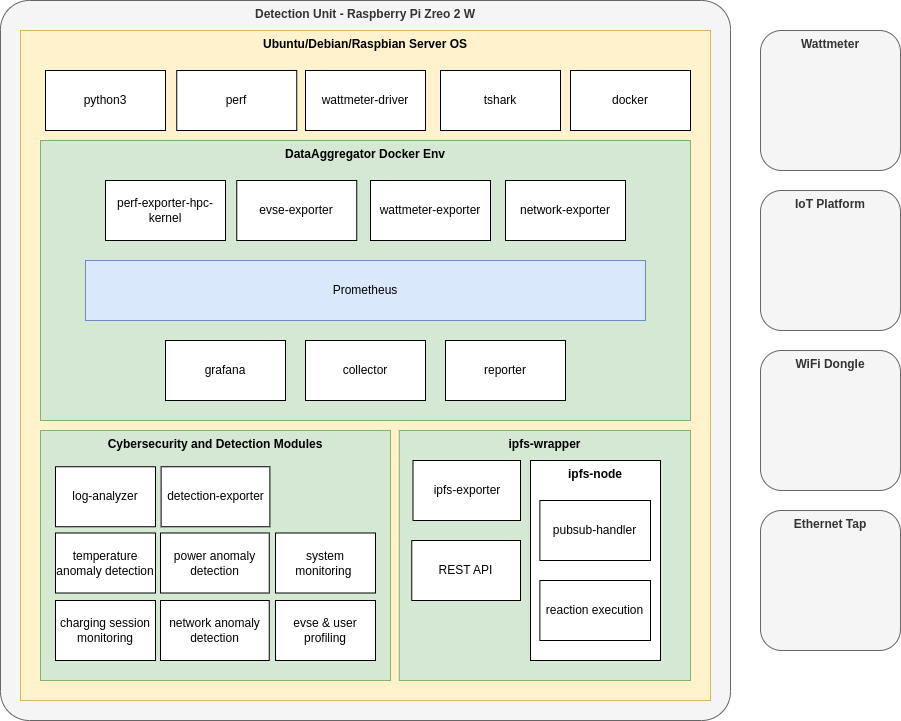
\includegraphics[width=\textwidth]{./figures/deployment_software_modules_v1.drawio.png}
    \caption{Gesamtarchitektur des ReSiLENT-Systems mit Charging Station
    und Cloud Dashboard}
    \label{fig:system_overview}
\end{figure}

Abbildung~\ref{fig:system_overview} zeigt die Gesamtarchitektur des Systems mit Fokus auf die in jeder Wallbox eingebettete Detektionseinheit. Als zentrales Laufzeitmodul fungiert der \textit{DataAggregator}, der die erfassten Sensordaten der Wallbox über Prometheus bereitstellt und sowohl den Cybersecurity- und Detektions-Modulen als auch Werkzeugen zur Datenaufbereitung zugänglich macht.

Die Architektur ist auf kollaborative Angriffserkennung ausgelegt: Über den \texttt{ipfs-wrapper} und dessen \textbf{Publish-Subscribe-Mechanismus} (detailliert in Abbildung~\ref{fig:ipfs_network} und~\ref{fig:dataflow}) teilen Ladesäulen Kontextinformationen mit allen Netzwerkteilnehmern und könnten somit die situative Wahrnehmung über die gesamte Ladeinfrastruktur hinweg verbessern.

\subsection{Privates IPFS-Netzwerk und Peer-to-Peer-Datenaustausch}

Für die verteilte Kommunikation zwischen den Detektionseinheiten und dem Cloud Dashboard wird ein privates IPFS-Netzwerk eingesetzt. Im Gegensatz
zum öffentlichen IPFS-Netz wird der Zugang durch einen gemeinsamen \textit{Swarm Key} beschränkt, sodass ausschließlich autorisierte Knoten dem Netzwerk beitreten können. Die Netzwerktopologie ist in Abbildung~\ref{fig:ipfs_network} dargestellt.

\begin{figure}[h]
    \centering
    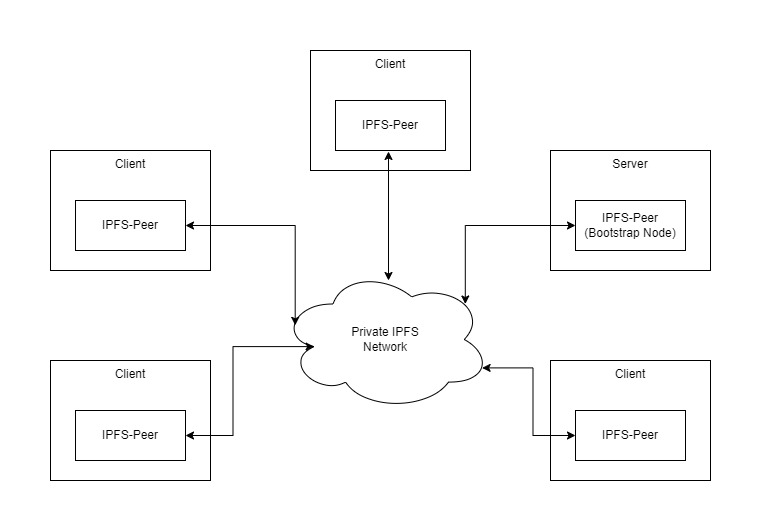
\includegraphics[width=0.75\textwidth]{./figures/Test-Mesh.jpg}
    \caption{Topologie des privaten IPFS-Netzwerks mit Bootstrap-Knoten und
    Client-Peers}
    \label{fig:ipfs_network}
\end{figure}

Der Netzbeitritt erfolgt über einen dedizierten \textbf{Bootstrap-Knoten}, der auf dem Server des Cloud Dashboards betrieben wird. Neue Peers melden
sich beim Bootstrap-Knoten an, erhalten die Multiaddresses (\textit{MADDR}) der bekannten Peers und kommunizieren anschließend direkt miteinander, ohne
den Bootstrap-Knoten als Relay zu verwenden. Jeder Knoten betreibt einen lokalen \textbf{IPFS-Peer-Daemon}, der über den \texttt{ipfs-wrapper}, wie in Abbildung~\ref{fig:dataflow} dargestellt, in die Systemarchitektur eingebunden ist.

Für die Benachrichtigung über neue Daten wird der
\textbf{Publish-Subscribe-Mechanismus} von IPFS genutzt: Sobald neue Messdaten erhoben werden, können diese veröffentlicht werden indem die Wallbox die zugehörige CID zusammen mit der eigenen MADDR über einen gemeinsam abonnierten Kanal an alle Teilnehmer versendet. Die Empfänger rufen die Datei daraufhin direkt beim Ursprungs-Peer ab. Da eine CID dem kryptografischen Hash des jeweiligen Inhalts entspricht, ist die Datenintegrität implizit gewährleistet, ohne dass zusätzliche Signaturmechanismen erforderlich sind.

\subsection{End-to-End-Datenfluss}

Der vollständige Datenfluss vom Sensor bis zur Visualisierung lässt sich in drei Phasen unterteilen: Datenerhebung und Aggregation auf der Charging Station, Transport über das IPFS-Netz sowie Persistierung und Darstellung im Cloud Dashboard. Das Sequenzdiagramm in Abbildung~\ref{fig:sequence} sowie der Datenfluss in Abbildung~\ref{fig:dataflow} illustrieren diesen Ablauf.

\begin{figure}[h]
    \centering
    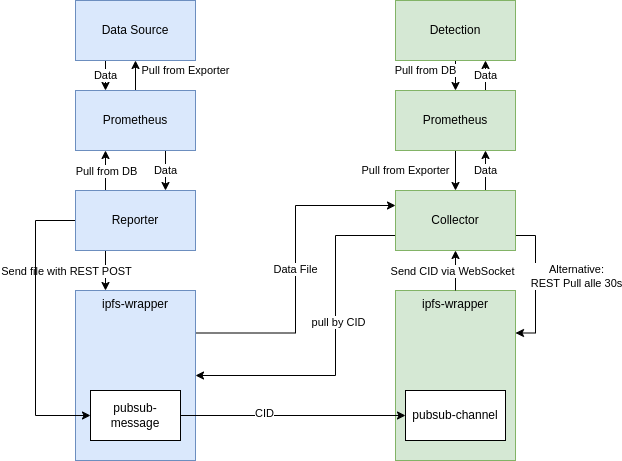
\includegraphics[width=\textwidth]{./figures/DataFlowIPFS.drawio.png}
    \caption{Datenfluss zwischen zwei Charging Stationen über IPFS}
    \label{fig:dataflow}
\end{figure}

\begin{figure}[h]
    \centering
    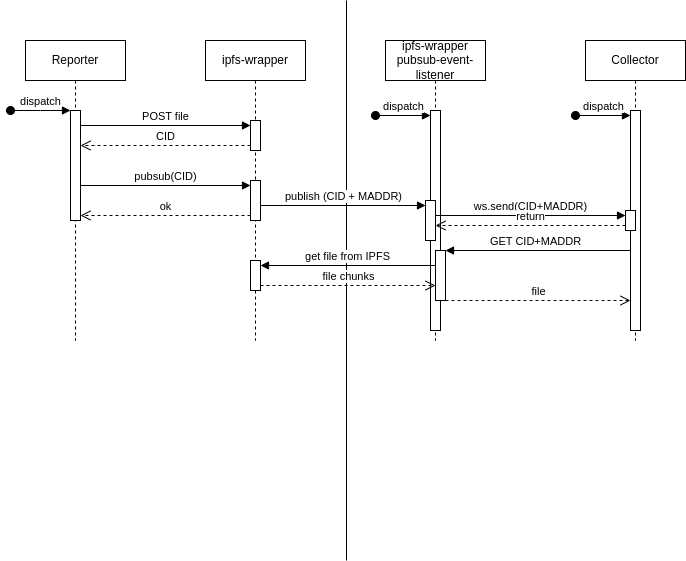
\includegraphics[width=0.85\textwidth]{./figures/Sequenzdiagramm_Datenfluss.drawio.png}
    \caption{Sequenzdiagramm des IPFS-basierten Datenaustausches}
    \label{fig:sequence}
\end{figure}

\paragraph{Datenerhebung (Charging Station)}
Der \textit{Aggregator} innerhalb des Knotens sammelt die Messdaten. Prometheus scraped alle Exporter in konfigurierbaren Intervallen. Der \textit{Reporter} liest die aggregierten Daten aus der Prometheus-Datenbank und übermittelt sie an den \texttt{ipfs-wrapper}.

\paragraph{Transport (IPFS-Netzwerk)}
Der \texttt{ipfs-wrapper} nimmt die Datei entgegen, publiziert sie im lokalen IPFS-Knoten und erhält eine CID zurück. Anschließend wird die CID zusammen mit der eigenen MADDR über den konfigurierten \textbf{Publish-Subscribe-Mechanismus} im privaten IPFS-Netz verbreitet. Die eigentlichen Messdaten werden dabei nicht aktiv gepusht, lediglich der Zeiger (CID) wird verteilt.

\paragraph{Persistierung und Visualisierung (Cloud Dashboard)}
Auf der Serverseite empfängt der \textit{Publish-Subscribe-Event-Listener} des \texttt{ipfs-wrapper} die CID und MADDR und leitet diese per \textbf{WebSocket} an den Collector weiter. Der Collector fordert daraufhin die vollständige Datei über den lokalen IPFS-Peer an, der sie in Chunks vom Ursprungs-Peer abruft. Der \textit{File Extractor} verarbeitet die Rohdaten und persistiert die Messwerte in \textbf{InfluxDB}. Grafana greift auf InfluxDB zu und stellt die Zeitreihendaten im Dashboard dar (siehe Abbildung~\ref{fig:cloud_dashboard}).

\begin{figure}[H]
    \centering
    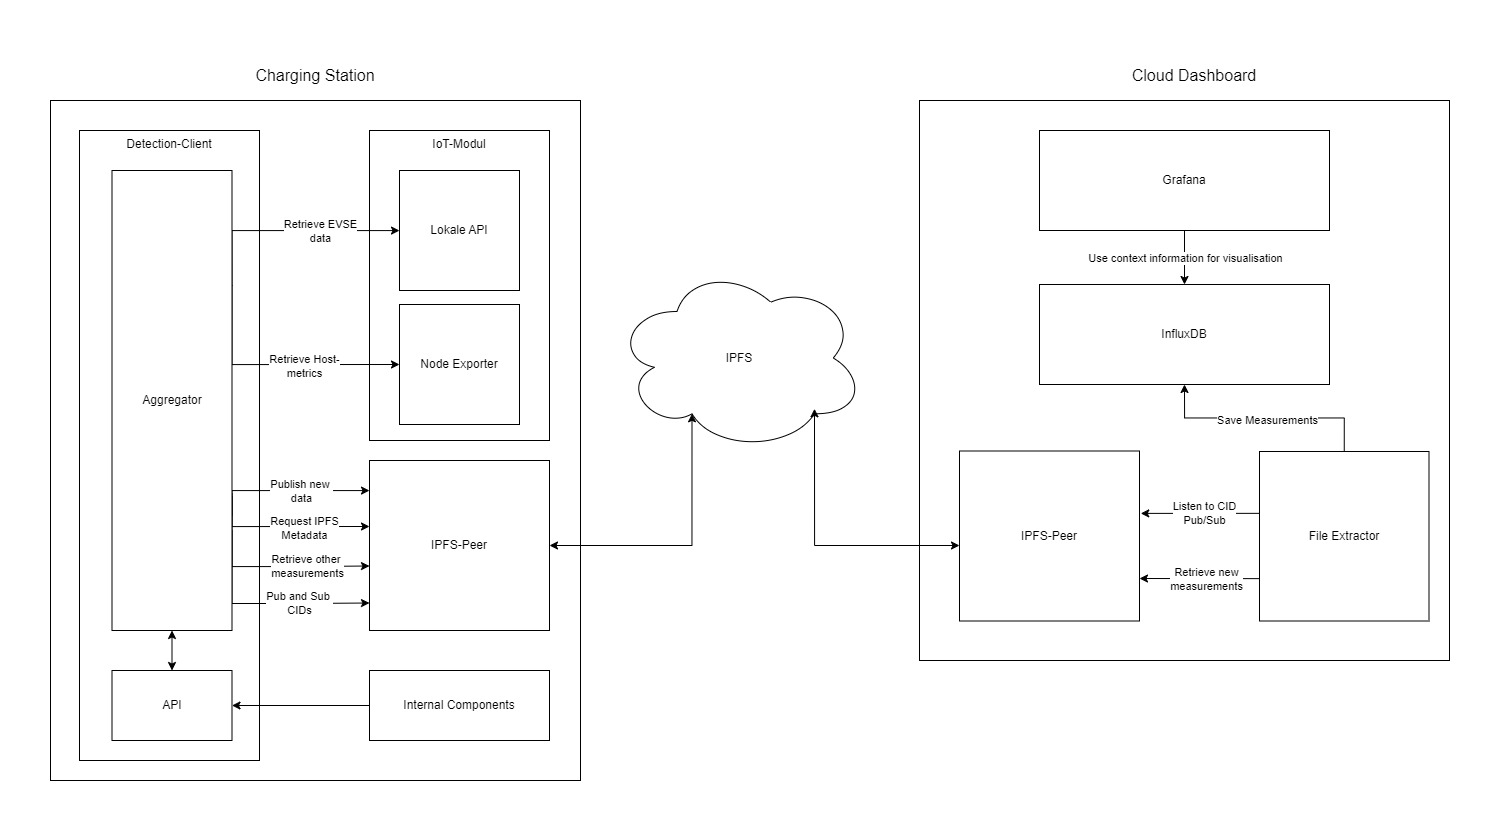
\includegraphics[width=0.75\textwidth]{./figures/System.jpg}
    \caption{Komponenten des Cloud Dashboards: IPFS-Peer, File Extractor, InfluxDB und Grafana}
    \label{fig:cloud_dashboard}
\end{figure}

Dieses Verständnis der Systemarchitektur und des Datenflusses bildet die Grundlage für die folgende Arbeit zur Implementierung des Threat-Reports und dessen spätere Aggregation. 